% -----------------------------------------------------------------------------------
%                               BIBLIOGRAPHY - Insert Name of BIB File Here
% -----------------------------------------------------------------------------------
\newpage

% ---------------BIBTEX OLD-----------------------------------------------------
% \bibliographystyle{unsrt} %%%% Plain or alpha can change orders here
% \bibliography{BibFile}
% \nocite{*} %%%if you want to see all references even those note cited in the text
% -----------------------------------------------------------------------------------

\printbibliography
% -----------------------------------------------------------------------------------
%                                  APENDIX
% -----------------------------------------------------------------------------------

% \end{counted} %<<<<<<<<<<<<<<ENDS WORD COUNTER

\newpage
\section{Appendices}

\subsection{Login Guide}
\subsubsection{Editor Login}

\begin{enumerate}

  \item Go to WordPress Login Page at http://ixn.host/wp-admin
  \item Use the Username: YunFu
  \item Use the Password: AppDesign
  \item View and edit Posts (news), Events, Projects and the Homepage (via Pages) content

\end{enumerate}

\subsubsection{Admin Login}
\begin{enumerate}

  \item Go to WordPress Login Page at http://ixn.host/wp-admin
  \item Use the Username: admin
  \item Use the Password: ixnTeam2017
  \item Access granted to all elements of the WordPress dashboard

\end{enumerate}

\subsubsection{Other Passwords}
\begin{itemize}

  \item \textbf{Vault:} password: ixnTeam2017. Make sure a new \textit{.vault\_pass} file is created when cloning the site repository with the password in the top line
  \item \textbf{Database:} User: admin , password: ixnTeam2017

\end{itemize}

///////////////

\subsection{WordPress Dashboard Guide}
\subsubsection{Update Home Page Content}

\begin{enumerate}

  \item Log in to WordPress Admin Account.
  \item Go to "Pages">"Home-Front Page"
  \item Update desired content

\end{enumerate}

\subsubsection{Update External Page Content}
\begin{enumerate}

  \item Log in to WordPress Admin Account.
  \item Go to "Pages"> Desired External Page
  \item Update desired content

\end{enumerate}

\subsubsection{Add News or Event Post}
\begin{enumerate}

  \item Log in to WordPress Admin Account
  \item Go to "News" or "Events" section
  \item Press "Add New"
  \item Enter post content

\end{enumerate}

\subsubsection{Add a Project}
\begin{enumerate}

  \item Log in to WordPress Admin Account.
  \item Go to "Projects" section
  \item Press "Add New"
  \item Enter title,decription,partner,authors,date,youtube video ID and select project catagory. (See image below for how to obtain youtube video ID)
  \item Add high resolution photo of project poster.
  \item Add high resolution "featured image" of the project. Please make sure you follow the guidelines below for uploading web or mobile featured images. It is essentail that you upload an image of the correct aspect ratio or the post will not appear well on the site. 

\end{enumerate}

 \begin{figure}[H]
      \centering
      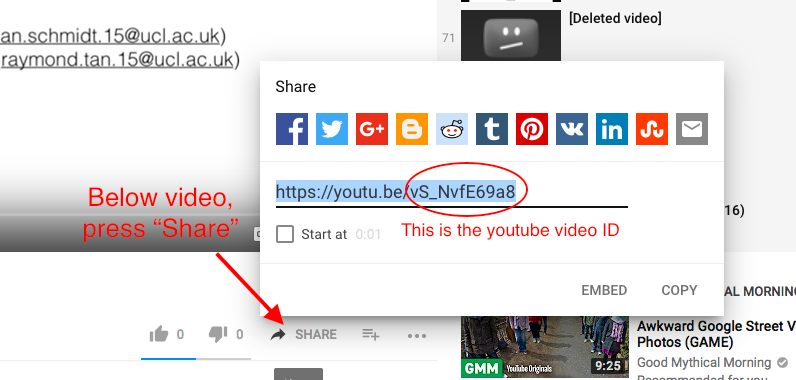
\includegraphics[trim = 0 0 0 0, clip, width=0.9\textheight]{vidpost.png}
      \caption{How to obtain youtube ID in order to add a project video on WordPress}
 \end{figure}

  \begin{figure}[H]
      \centering
      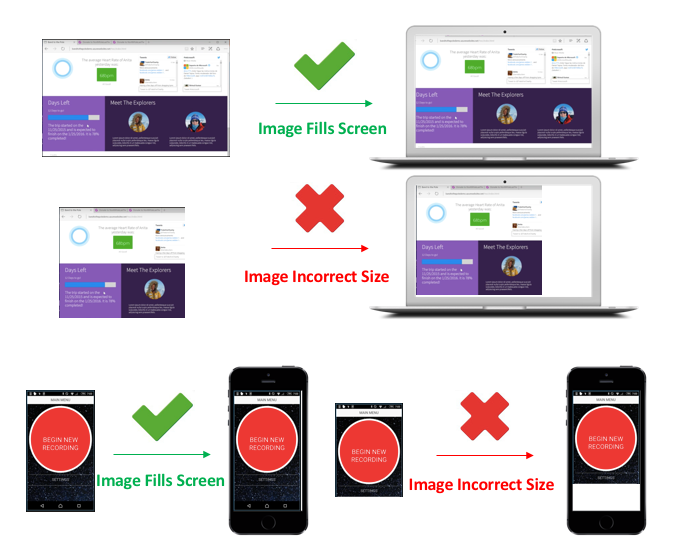
\includegraphics[trim = 0 0 0 0, clip, width=0.9\textheight]{screenimg.png}
      \caption{It is essentail to upload a featured image of the correct size in order to maintain the look of the site.}
 \end{figure}

//////////////////

\begin{landscape}
\subsection{Competing Solutions}
  \begin{table}[H]
      \centering
      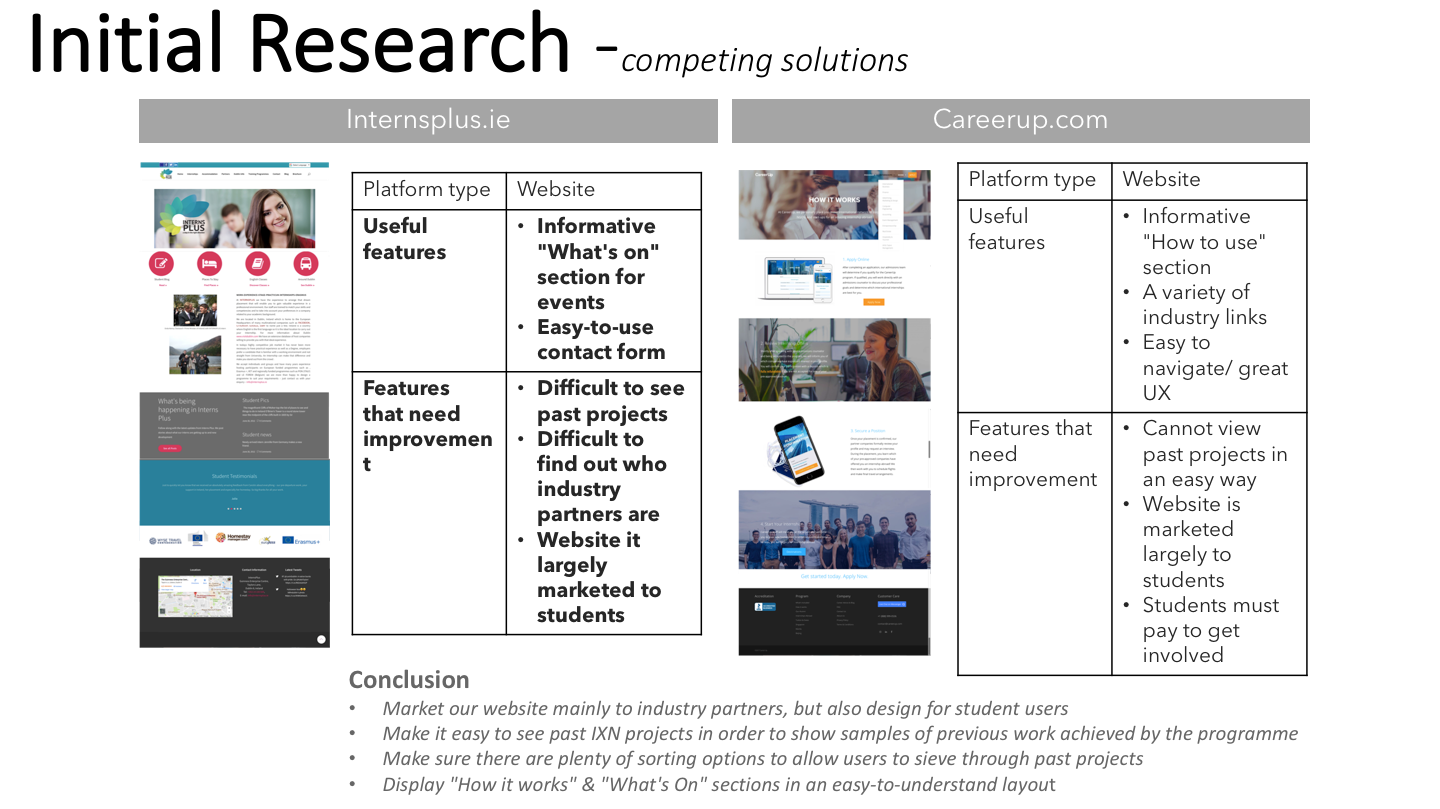
\includegraphics[trim = 0 0 0 0, clip, width=1.3\textheight]{app5.png}
      \caption{Possible features to be implemented in the future}
 \end{table}
 \end{landscape}

 \newpage


\begin{landscape}
\subsection{Sketches}
 \begin{figure}[H]
      \centering
      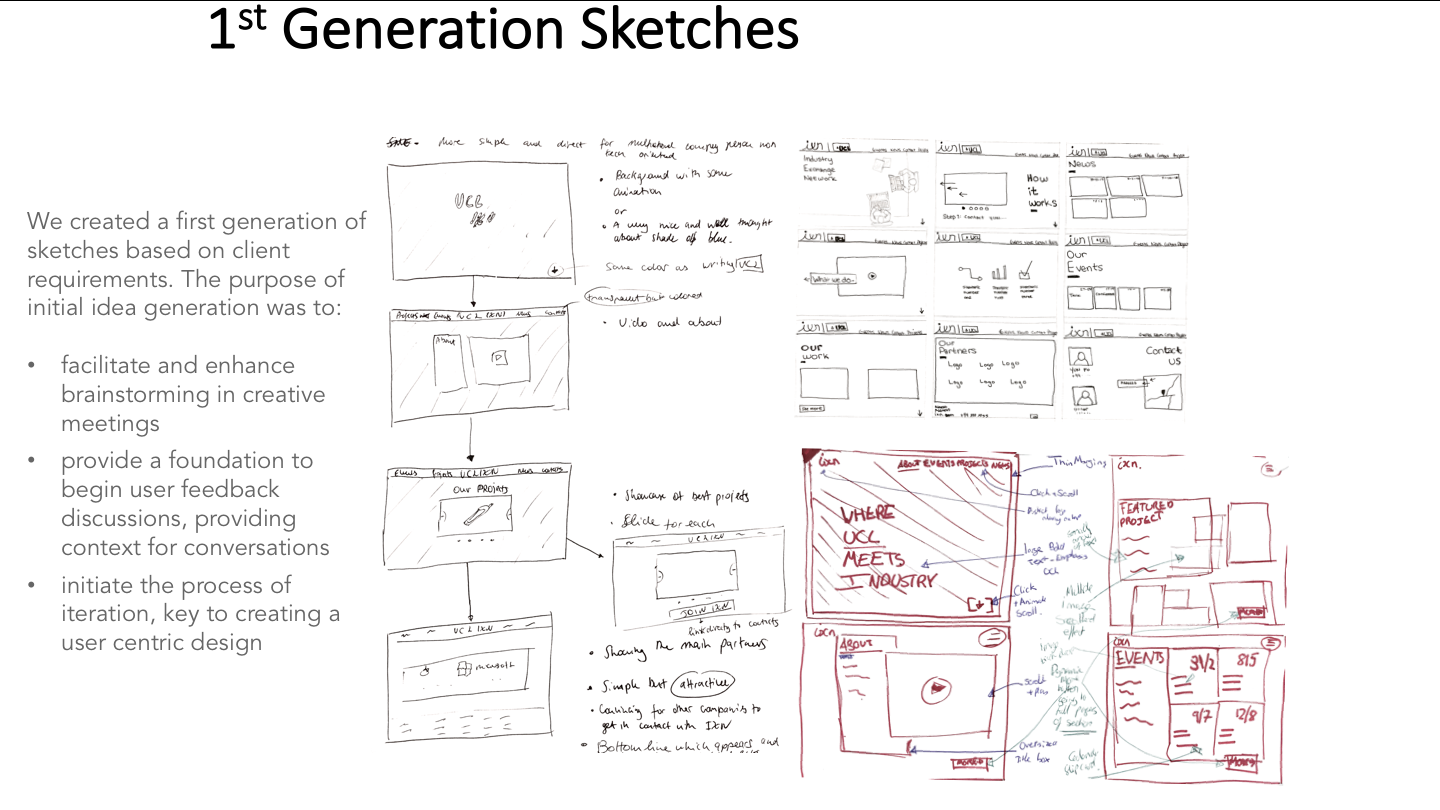
\includegraphics[trim = 0 0 0 0, clip, width=1.3\textheight]{app4.png}
      \caption{First generation hand-drawn sketches}
 \end{figure}
\end{landscape}

 \newpage

\begin{landscape}
 \begin{figure}[H]
      \centering
      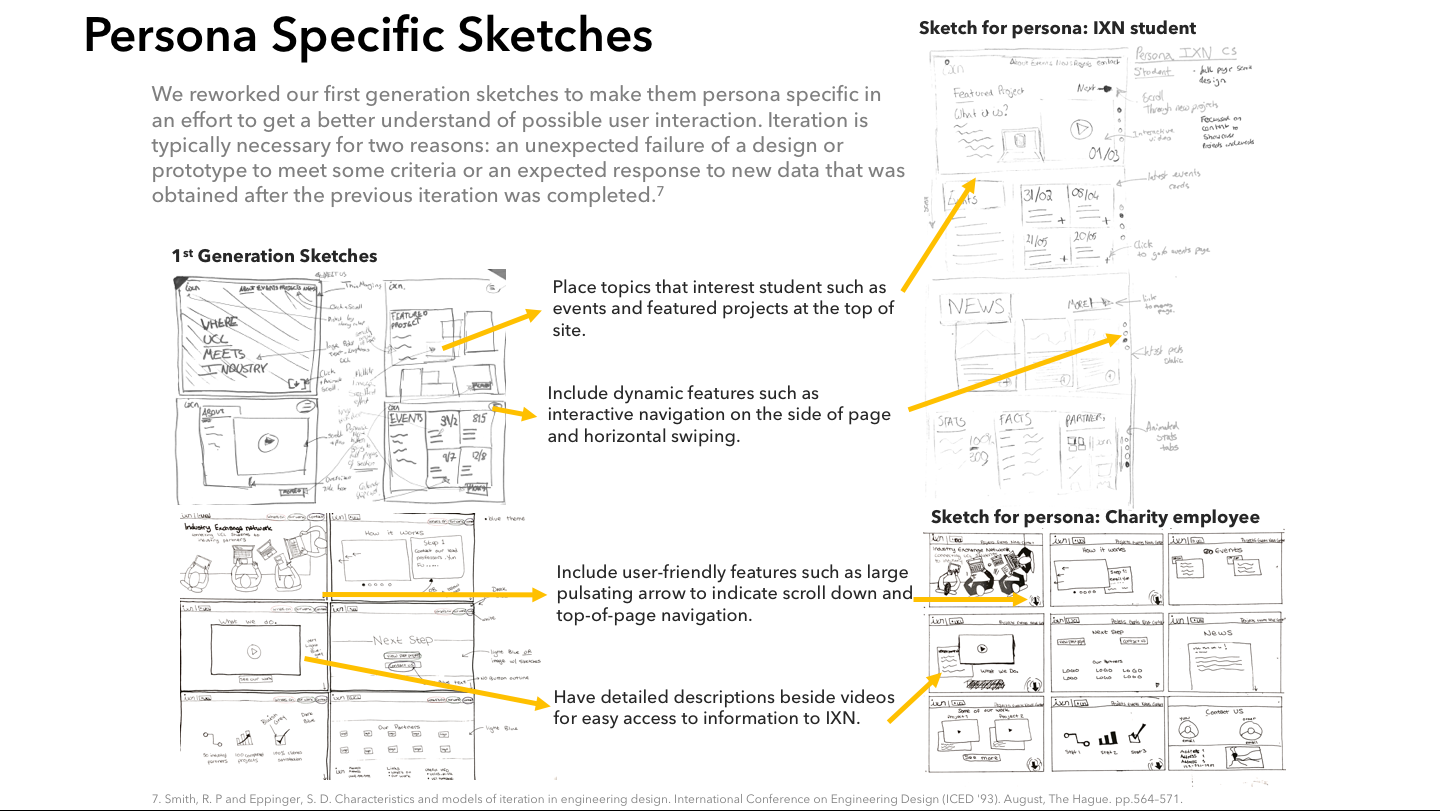
\includegraphics[trim = 0 0 0 0, clip, width=1.3\textheight]{app3.png}
      \caption{Sketches based on researched personas}
 \end{figure}
  \end{landscape}

\newpage

\begin{landscape}
\subsection{Storyboards}
 \begin{figure}[H]
      \centering
      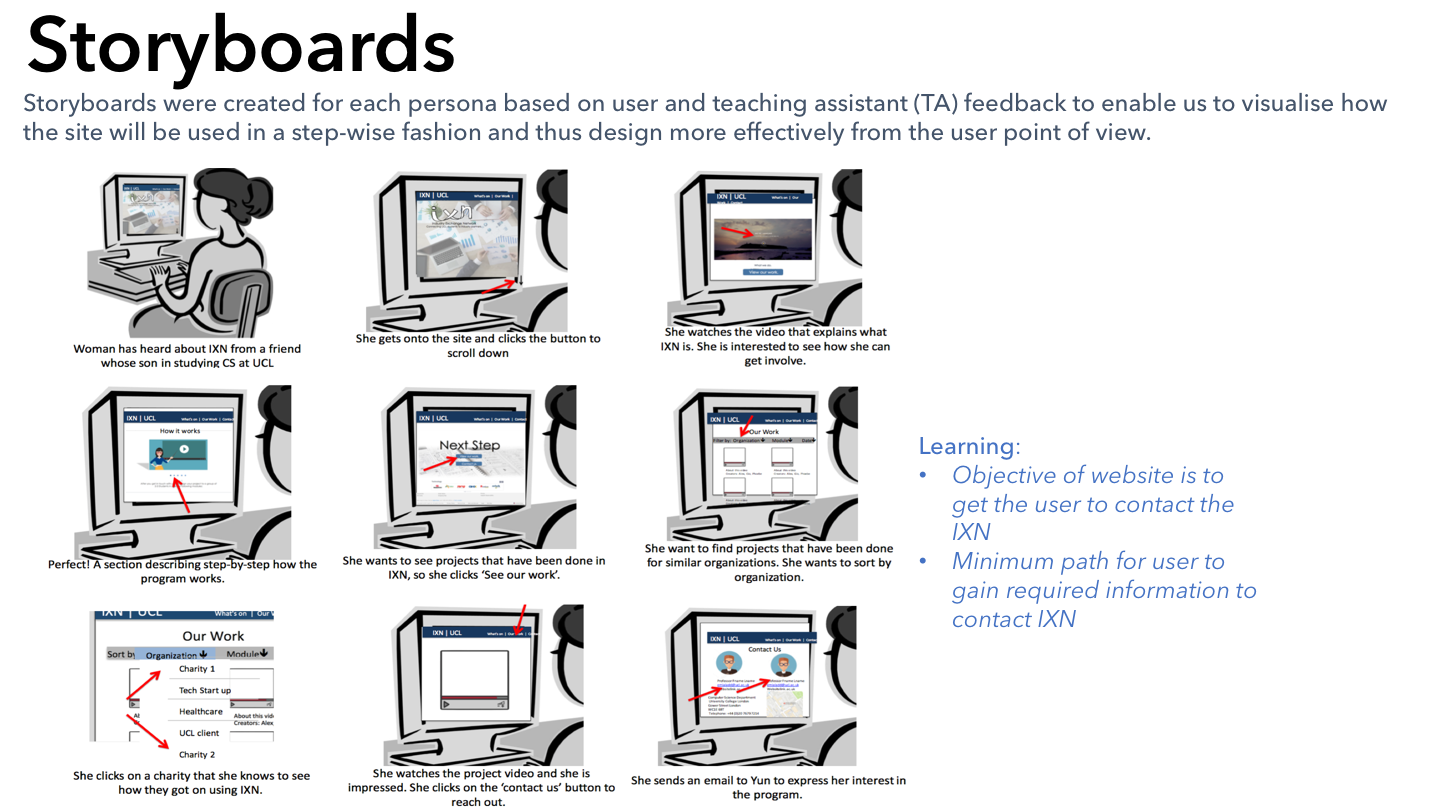
\includegraphics[trim = 0 0 0 0, clip, width=1.3\textheight]{app2.png}
      \caption{Storyboard example describing a possible user experience}
 \end{figure}

 \newpage

\subsection{Wire-Framing}
\begin{table}[H]
      \centering
      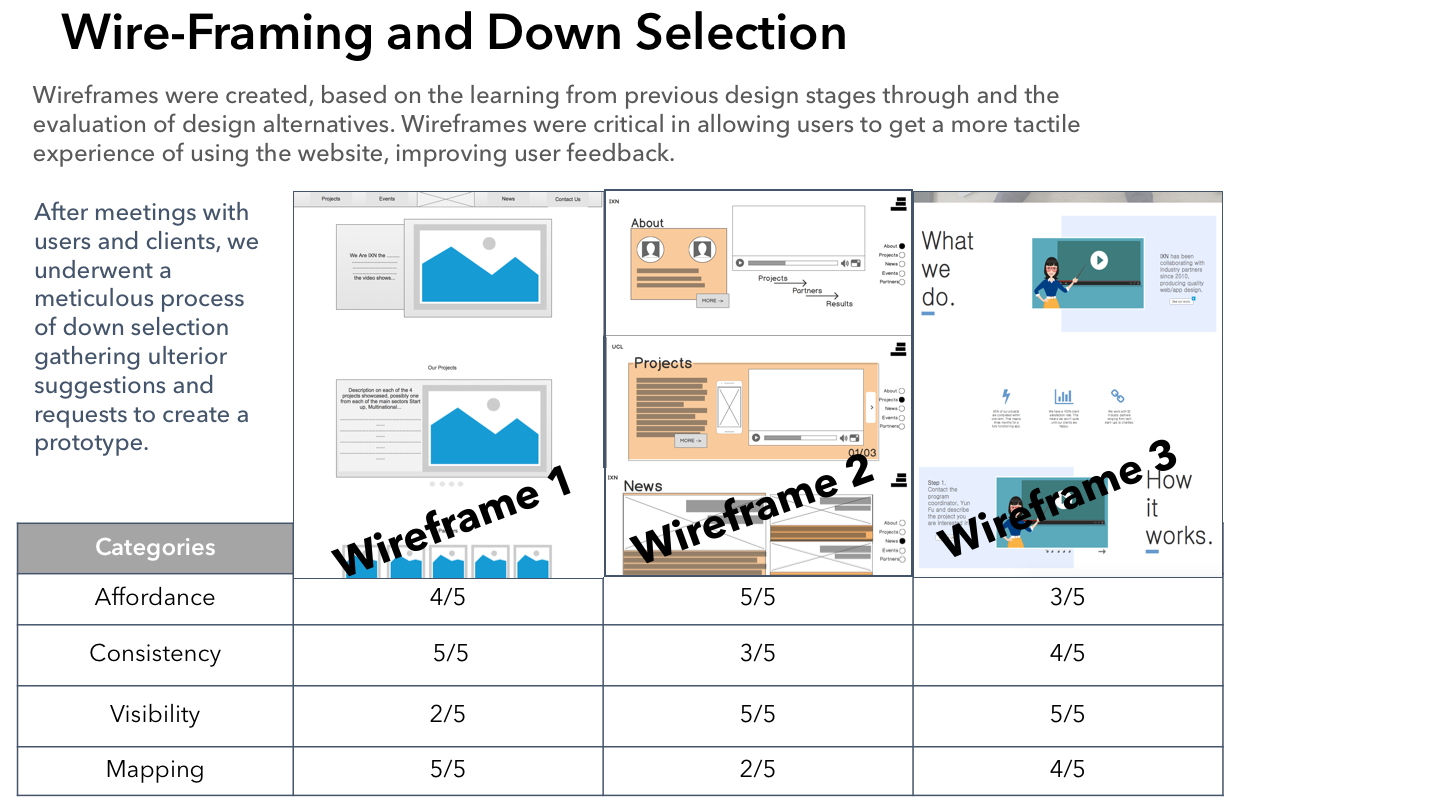
\includegraphics[trim = 0 0 0 0, clip, width=1.3\textheight]{app1.png}
      \caption{Down selection of wire-frames}
 \end{table}
  \end{landscape}
\subsection{IXN Poll}
\begin{figure}[H]
      \centering
      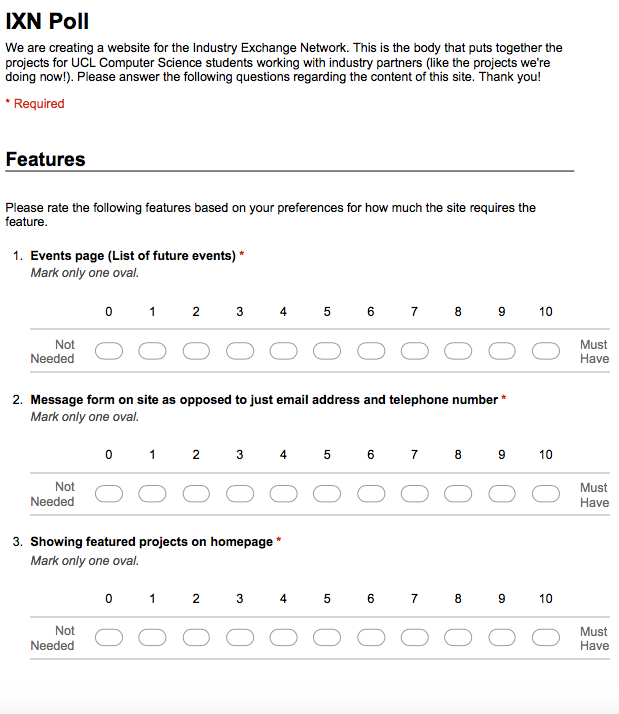
\includegraphics[trim = 0 0 0 0, clip, width=0.99\textwidth]{Poll1.png}
      \caption{IXN poll example page 1.}
 \end{figure}

 \begin{figure}[H]
      \centering
      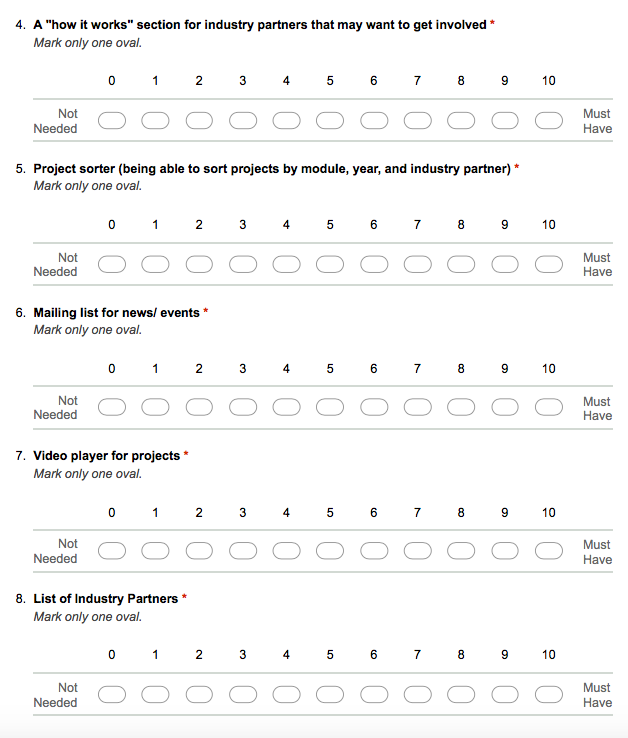
\includegraphics[trim = 0 0 0 0, clip, width=0.99\textwidth]{Poll2.png}
      \caption{IXN poll example page 2.}
 \end{figure}

 \begin{figure}[H]
      \centering
      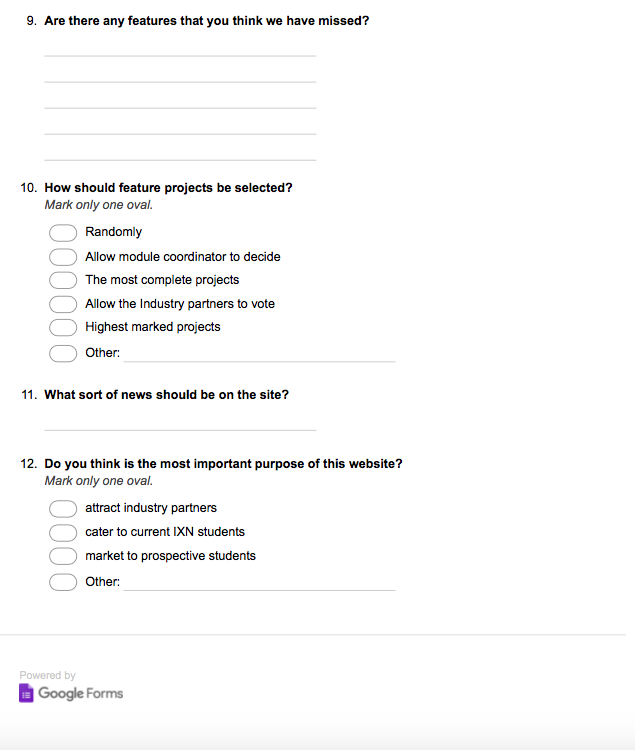
\includegraphics[trim = 0 0 0 0, clip, width=0.99\textwidth]{Poll3.png}
      \caption{IXN poll example page 3.}
 \end{figure}

\subsection{IXN-Poll-Results}
\begin{figure}[H]
      \centering
      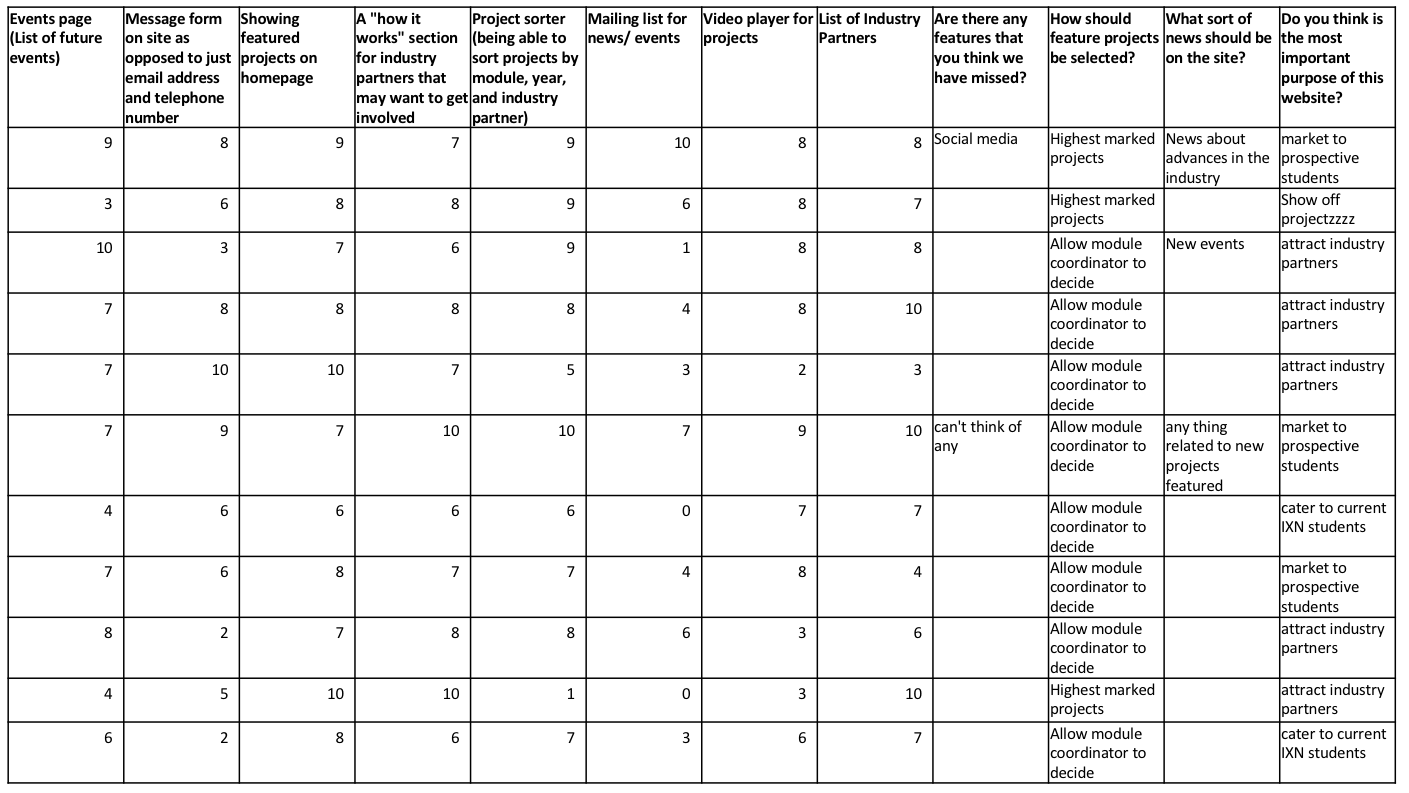
\includegraphics[trim = 0 0 0 0, clip, width=0.99\textwidth]{PollResults.png}
      \caption{Down selection of wire-frames.}
 \end{figure}


 \newpage

\subsection{Known Bugs}
 \begin{table}[H]
      \centering
      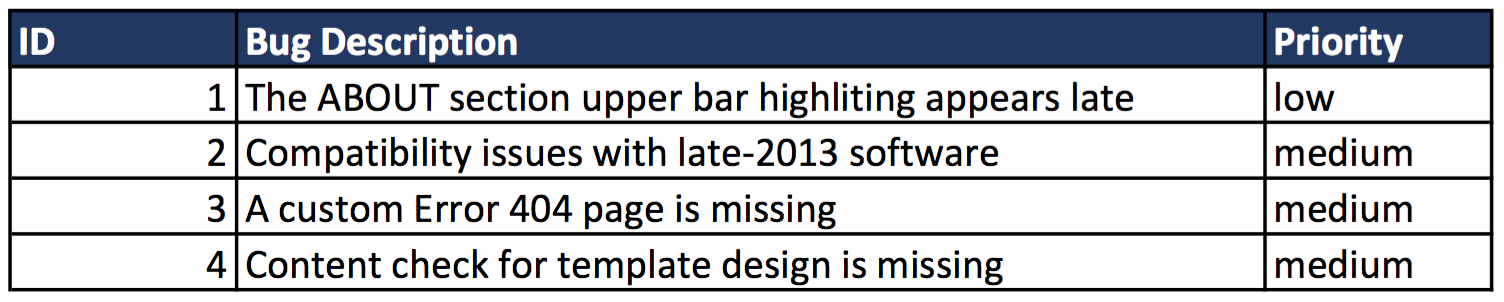
\includegraphics[trim = 0 0 0 0, clip, width=0.99\textwidth]{App7.png}
      \caption{Know bugs description and importance}
 \end{table}


\end{document}